
\documentclass[xcolor={dvipsnames}]{beamer}
\usepackage{amsmath,amsfonts,amssymb,pxfonts,eulervm,xspace}
\usepackage{graphicx}
 \usepackage{multimedia}
\usepackage{media9}
\usepackage{minted}
\usepackage{mathtools}

\usepackage{animate}

\graphicspath{{./figures/}}
\usetheme{ccnycrest}


\begin{document}

\title{ CS102: Functions }
\author{Hannah Aizenman}

\begin{frame}
	\titlepage
\end{frame}

\begin{frame}[plain]
		\begin{figure}
	\includegraphics[width=.9\textwidth]{function}
		\end{figure}
\end{frame}
\begin{frame}{$f(x)=x^{2}$}
	\includegraphics[width=1\textwidth]{xsq}
\end{frame}

\begin{frame}{Using Functions}
	\begin{center}
	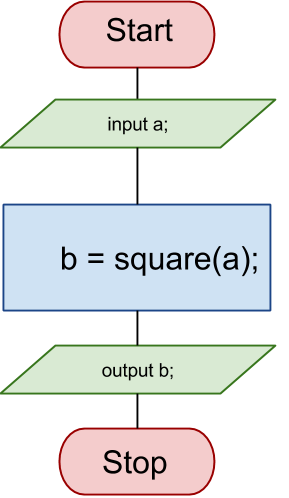
\includegraphics[width=.4\textwidth]{fsq}
	\end{center}
\end{frame}

\begin{frame}{Using Functions}
	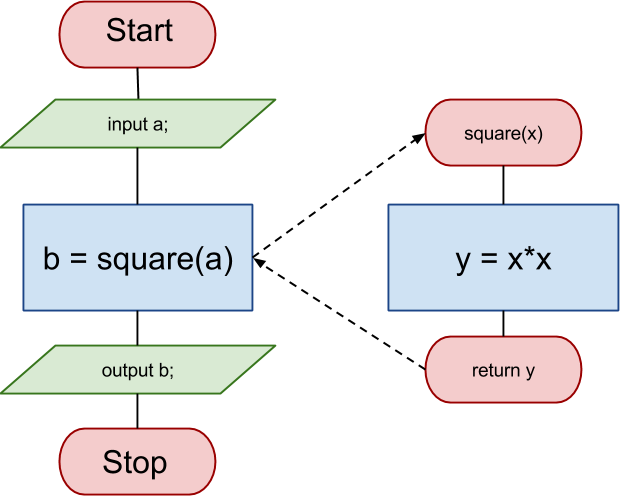
\includegraphics[width=1\textwidth]{fsq_function}
\end{frame}

\begin{frame}[fragile]{Implementing square(x)}
	\begin{center}
	 
	\begin{minted}{c++}
	//prototype
	int square(int x);

	//implementation
	int square(int x){
	   int y = x*x;
	   return y;
	}   
	\end{minted}
	\end{center}
	\begin{center}
		\begin{itemize}
			\item function and return \textbf{must} have same type
			\item parameters can be of various types
			\item use descriptive names, like square instead of f
		\end{itemize}
	\end{center}
\end{frame}

\begin{frame}{ Pass-by-Value}
	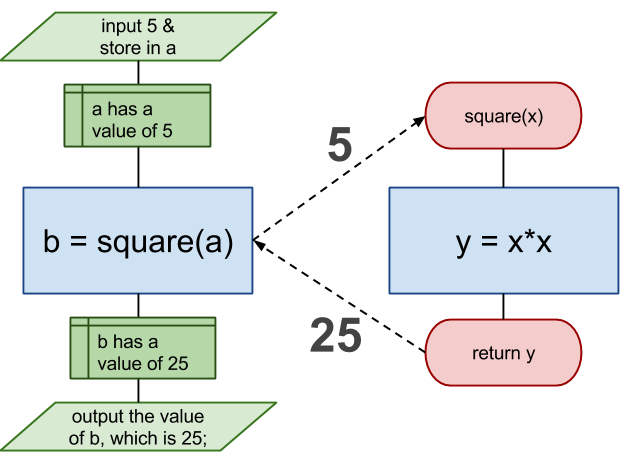
\includegraphics[width=1\textwidth]{fsq_pbv}
\end{frame}

\begin{frame}[fragile]{Using square(x)}
	\begin{minted}{c++}
#include <iostream>

int square(int x); //function prototype

int main(){
    int a;
    std::cin>>a;
    int b = square(a);
    std::cout<<"square("<<a<<")="<<b<<std::endl;
    return 0;
}
//computes x^2
int square(int x){
    int y = x*x;
    return y;
}   
	\end{minted}
\end{frame}

\begin{frame}{practice}
	\begin{itemize}
		\item Write a function named check() that has three parameters. The first parameter should accept an integer number, and the second and third parameters should accept a double-precision number. The function body should display the values of
data passed to the function.
		\item Write a function named rightTriangle() that accepts the lengths of two sides of a right triangle as the arguments a and b. The function should determine and return the hypotenuse, c, of the triangle.
	\end{itemize}
\end{frame}

\begin{frame}[fragile]{Pass by reference: square(x)}
	\begin{center} 
	\begin{minted}{c++}
	//prototype
	void square(int x, int &y);

	//implementation
	void square(int x, int &y){
	   y = x*x;
	}   
	\end{minted}
	\end{center}
	\begin{center}
		\begin{itemize}
			\item reference parameters are pointers
			\item a function of type void doesn't return anything
			\item a function can have pass by value and pass by reference parameters
		\end{itemize}
	\end{center}
\end{frame}

\begin{frame}{Pass-by-Reference}
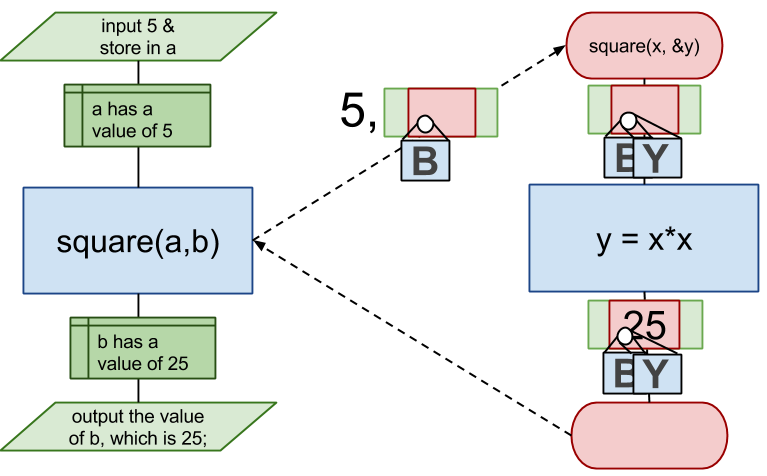
\includegraphics[width=1\textwidth]{fsq_pbr}
\end{frame}

\begin{frame}[fragile]{Using square(x)}

\begin{minted}{c++}
#include <iostream>

void square(int x, int &y); //function prototype

int main(){
    int a, b;
    std::cin>>a;
    square(a, b);
    std::cout<<"square("<<a<<")="<<b<<std::endl;
    return 0;
}
//function for computing x^2
void square(int x, int &y){
    y = x*x;
}   
\end{minted}

\end{frame}

\begin{frame}{practice}
	\begin{itemize}
		\item implement the function addn that adds some value n to an input parameter x. The user can set n, but it defaults to 0.
		\item write a function to sort 3 values and return the sorted values
	\end{itemize}
\end{frame}

\begin{frame}[fragile]{Default Args}
	\begin{center}
	\begin{minted}{c++}
	//prototype
	int square(int x=0);

	//implementation
	int square(int x=0){
	   int y = x*x;
	   return y;
	}   
	\end{minted}
	\end{center}
	\begin{center}
	\begin{itemize}
		\item function can have unlimited number of parameters
		\item function can have unlimited number of default args
		\item defaults must come after regular parameters
	\end{itemize}
	\end{center}
\end{frame}

\begin{frame}[fragile]{Default Args: using square(x)}

\begin{minted}{c++}
#include <iostream>

int square(int x=0);

int main(){
   std::cout<<"square(0)="<<square()<<std::endl;
   return 0;
}

int square(int x=0){
    int y = x*x;
    return y;
}   
\end{minted}

\end{frame}

\begin{frame}{practice}
	\begin{itemize}
		\item modify check() so that the last value defaults to 42
		\item modify rightTriangle() so that if a side isn't intered, it's set as 0
	\end{itemize}
\end{frame}

\begin{frame}[fragile]{Overloading}

	\begin{columns}
	\begin{column}{.49\textwidth}
	\begin{minted}{c++}
	//prototypes
	int square(int x);
	double square(double x);
	
	//implementation
	int square(int x){
	   int y = x*x;
	   return y;
	}
   
	double square(double x){
	   double y = x*x;
	   return y;
	}   
	\end{minted}
	\end{column}
	\begin{column}{.49\textwidth}
	\begin{itemize}
		\item can overload based on parameter type
		\item can also overload based on parameter count
	\end{itemize}
	\end{column}
	\end{columns}
\end{frame}


\begin{frame}[fragile]{Overloading: using square(x)}
	\begin{minted}{c++}
	int square(int x);
	double square(double x);

	int main(){
	   int w = square(2);
	   std::cout<<"square(2)="<<w<<std::endl;
	   double v = square(2.5);
	   std::cout<<"square(2.5)="<<v<<std::endl;
	   return 0;
	}
//implementations
\end{minted}
\end{frame}

\begin{frame}{practice}
	\begin{itemize}
		\item overload check to accept all ints
		\item overload rightTriangle() to accept doubles
	\end{itemize}
\end{frame}

\begin{frame}[fragile]{Templates}
	\begin{center} 
	\begin{minted}{c++}
template <class T>
T square(T x){
    T y;
    y = x*x;
    return y;
}   
	\end{minted}
	\end{center}
	\begin{center}
		\begin{itemize}
			\item the function implementation \textbf{is} the prototype
			\item custom function created on function call
			\item T is a stand in for any built in data type
			\item Can be pass-by-value and/or pass-by-reference	
		\end{itemize}
	\end{center}
\end{frame}

\begin{frame}[fragile]{Templates: Multiple types}
	\begin{center} 
	\begin{minted}{c++}
template <class T1, class T2>
void square(T1 x, T2 &y){
    y = x*x;
}   
	\end{minted}
	\end{center}
	\begin{center}
		\begin{itemize}
			\item T1 and T2 are different types
			\item function doesn't have to return a templated type
			\item function can return template type
			\item Can be pass-by-value and/or pass-by-reference
			\item T1, T2...are a convention, can be anything
		\end{itemize}
	\end{center}
\end{frame}

\begin{frame}[fragile]{Using Templates}
\begin{minted}{c++}
#include <iostream>

template <class T>
T square(T x){
    y = x*x;
}

int main(){
   int w = square(2);
   std::cout<<"square(2)="<<w<<std::endl;
   double v = square(2.5);
   std::cout<<"square(2.5)="<<v<<std::endl;
   return 0;
}
\end{minted}
\end{frame}


\begin{frame}{Variable Scope}
	\begin{itemize}
		\item local scope
		\begin{itemize}
			\item only seen by function it's defined in
			\item name can be reused in other functions
		\end{itemize}
		\item global scope
		\begin{itemize}
			\item entire program can see the variable
			\item defined outside main
			\item bad practice-don't use unless required
		\end{itemize}
	\end{itemize}
\end{frame}

\begin{frame}[fragile]{Variable storage allocation}
	\begin{minted}{c++}
		auto int var1;
		static int var2;
		extern int var3;
	\end{minted}
	\begin{description}
		\item[auto (default)] storage allocated on execution
		\item[static] storage allocated on compilation
		\item[extern] storage can be seen by other files
	\end{description}
\end{frame}

\end{document}

